\chapter{Revisão Bibliográfica} \label{RevisaoBibliografica}

% Palavras-chave dos algoritmos em português
\SetKwInput{KwIn}{Entrada}
\SetKwInput{KwOut}{Saída}
\SetKwFor{For}{para}{faça}{fim}
\SetKwFor{ForEach}{para cada}{faça}{fim}
\SetKw{Return}{retorna}
\SetAlgorithmName{Algoritmo}{algoritmo}{Lista de Algoritmos}

Este capítulo reúne os conceitos necessários para compreender o problema investigado e apresenta o que outros autores já estudaram sobre o tema. A Seção~\ref{sec:fundamentacao} constrói a base teórica passo a passo: começa pelo modo como uma rede neural aprende, passa pelo aprendizado federado e pelos ataques que exploram os gradientes, e termina nas defesas e nas métricas usadas para avaliá-las. Para tornar os conceitos mais concretos, um mesmo exemplo numérico, chamado aqui de exemplo guia, acompanha o leitor ao longo de toda a seção. A Seção~\ref{sec:relacionados} descreve os trabalhos relacionados e posiciona esta pesquisa em relação a eles.

% =====================================================================
\section{Fundamentação Teórica} \label{sec:fundamentacao}
% =====================================================================

\subsection{Aprendizado de Máquina Supervisionado}

O termo aprendizado, no contexto do aprendizado de máquina, refere-se à melhora de desempenho obtida por meio da experiência. Da mesma forma que um estudante melhora suas notas à medida que resolve mais exercícios, um programa de computador pode melhorar suas previsões à medida que analisa mais dados. \citeonline{Mitchell1997} formaliza essa ideia: um programa aprende a partir de uma experiência $E$, com respeito a uma tarefa $T$ e a uma medida de desempenho $P$, se seu desempenho em $T$, medido por $P$, melhora com $E$. Neste trabalho, a tarefa é classificar imagens, a experiência é um conjunto de imagens já rotuladas e o desempenho é a proporção de acertos em imagens que o modelo nunca viu.

Quando cada exemplo vem acompanhado da resposta correta, como uma foto acompanhada da etiqueta ``gato'', o problema é chamado de aprendizado supervisionado. Formalmente, dispõe-se de um conjunto de dados $\mathcal{D} = \{(x_i, y_i)\}_{i=1}^{N}$, em que $x_i$ é a entrada (os pixels de uma imagem) e $y_i \in \{1, \dots, K\}$ é a classe correspondente. Treinar o modelo significa encontrar os parâmetros $\theta$ de uma função $f_\theta$ que errem o mínimo possível nesses exemplos, ou seja, que minimizem o risco empírico \cite{Goodfellow2016}:

\begin{equation} \label{eq:risco}
\theta^{*} = \arg\min_{\theta} \; \mathcal{L}(\theta) = \arg\min_{\theta} \; \frac{1}{N} \sum_{i=1}^{N} \ell\big(f_\theta(x_i), y_i\big)
\end{equation}

\noindent onde:
\begin{description}
  \item[$\theta$] = vetor de parâmetros (pesos) do modelo;
  \item[$f_\theta(x_i)$] = saída do modelo para a entrada $x_i$;
  \item[$\ell$] = função de perda, que mede o quanto a previsão se afasta da resposta correta;
  \item[$N$] = número de exemplos de treinamento.
\end{description}

Em problemas de classificação com $K$ classes, a rede produz um vetor de pontuações $z \in \mathbb{R}^{K}$, chamadas logits, uma para cada classe. A função softmax transforma essas pontuações em probabilidades, e a perda mais utilizada é a entropia cruzada, que penaliza o modelo quando ele atribui baixa probabilidade à classe correta:

\begin{equation} \label{eq:softmax-ce}
p_j = \frac{e^{z_j}}{\sum_{k=1}^{K} e^{z_k}}, \qquad \ell(z, c) = -\log p_c
\end{equation}

\noindent onde:
\begin{description}
  \item[$p_j$] = probabilidade atribuída pelo modelo à classe $j$;
  \item[$c$] = índice da classe correta.
\end{description}

Se o modelo atribui probabilidade $0{,}9$ à classe correta, a perda é $-\log 0{,}9 \approx 0{,}11$; se atribui apenas $0{,}1$, a perda sobe para $-\log 0{,}1 \approx 2{,}30$. Essa estrutura da entropia cruzada será explorada mais adiante pelos ataques de inferência de rótulo (Seção~\ref{sec:idlg}).

\subsection{Treinamento de Redes Neurais por Gradiente} \label{sec:gradiente}

Para redes neurais, a Equação~\ref{eq:risco} não tem solução direta, e os parâmetros precisam ser ajustados aos poucos. A ideia pode ser comparada a descer uma montanha no escuro: sem enxergar o vale, a pessoa sente a inclinação do terreno sob os pés e dá um passo na direção em que ele desce. Em aprendizado de máquina, essa inclinação é o gradiente $\nabla_\theta \mathcal{L}$, que indica a direção em que a perda mais cresce; basta, portanto, caminhar no sentido oposto.

Como calcular o gradiente sobre todos os exemplos a cada passo seria muito custoso, utiliza-se o gradiente descendente estocástico (SGD), que estima o gradiente a partir de um pequeno lote (batch) de exemplos sorteados:

\begin{equation} \label{eq:sgd}
\theta_{t+1} = \theta_t - \eta \, g_t, \qquad g_t = \frac{1}{B} \sum_{i \in \mathcal{B}_t} \nabla_\theta \, \ell\big(f_{\theta_t}(x_i), y_i\big)
\end{equation}

\noindent onde:
\begin{description}
  \item[$\eta$] = taxa de aprendizado, que controla o tamanho do passo;
  \item[$\mathcal{B}_t$] = lote de exemplos sorteado na iteração $t$;
  \item[$B$] = tamanho do lote;
  \item[$g_t$] = gradiente médio calculado sobre o lote.
\end{description}

Como ilustração, considere a função $\mathcal{L}(\theta) = \theta^2$, cujo mínimo está em $\theta = 0$, com gradiente $2\theta$, ponto inicial $\theta_0 = 3$ e taxa $\eta = 0{,}1$. O primeiro passo resulta em $\theta_1 = 3 - 0{,}1 \times 6 = 2{,}4$; o segundo, em $\theta_2 = 2{,}4 - 0{,}1 \times 4{,}8 = 1{,}92$. A cada iteração, o parâmetro se aproxima do mínimo. Em uma rede neural, o mesmo processo ocorre simultaneamente para milhões de parâmetros, e o gradiente de cada um é obtido de forma eficiente pelo algoritmo de retropropagação (backpropagation), que aplica a regra da cadeia da saída para a entrada da rede \cite{Rumelhart1986}.

Na prática, é comum usar variações do SGD. Uma das mais populares é o otimizador Adam \cite{Kingma2015}, que ajusta automaticamente o tamanho do passo de cada parâmetro com base em médias móveis do gradiente e de seu quadrado:

\begin{equation} \label{eq:adam}
\begin{aligned}
m_t &= \beta_1 m_{t-1} + (1-\beta_1)\, g_t, & \hat{m}_t &= \frac{m_t}{1-\beta_1^{t}}, \\
v_t &= \beta_2 v_{t-1} + (1-\beta_2)\, g_t^{2}, & \hat{v}_t &= \frac{v_t}{1-\beta_2^{t}}, \\
\theta_{t+1} &= \theta_t - \eta \, \frac{\hat{m}_t}{\sqrt{\hat{v}_t} + \epsilon}
\end{aligned}
\end{equation}

\noindent onde:
\begin{description}
  \item[$m_t$, $v_t$] = médias móveis do gradiente e do gradiente ao quadrado;
  \item[$\hat{m}_t$, $\hat{v}_t$] = versões dessas médias corrigidas para o início do treinamento;
  \item[$\beta_1$, $\beta_2$] = taxas de decaimento (tipicamente $0{,}9$ e $0{,}999$);
  \item[$\epsilon$] = constante pequena que evita divisão por zero.
\end{description}

A vantagem do Adam é convergir bem sem exigir um ajuste cuidadoso da taxa de aprendizado; em contrapartida, armazena duas médias adicionais por parâmetro, o que aumenta o uso de memória.

\subsubsection{O Gradiente Carrega Informação sobre os Dados}

Um ponto central para este trabalho é que o gradiente depende diretamente dos dados usados para calculá-lo. Considere uma camada totalmente conectada $z = Wa + b$, que recebe um vetor $a$ e produz as pontuações $z$. Pela regra da cadeia, o gradiente da perda em relação aos pesos e ao viés da $i$-ésima saída é:

\begin{equation} \label{eq:grad-linear}
\frac{\partial \ell}{\partial W_{i}} = \frac{\partial \ell}{\partial z_i} \, a^{\top}, \qquad \frac{\partial \ell}{\partial b_i} = \frac{\partial \ell}{\partial z_i}
\end{equation}

\noindent ou seja, cada linha do gradiente dos pesos é uma cópia da entrada $a$ multiplicada por um número. Para ver o que isso significa na prática, considere o exemplo a seguir, que será reutilizado ao longo de todo o capítulo.

O exemplo guia consiste em um modelo com uma única camada linear que classifica entradas em três classes: avião, gato e navio. A entrada é um vetor com quatro valores não negativos, $a = (0{,}5;\ 1{,}0;\ 0{,}2;\ 2{,}0)$, que pode ser entendido como quatro características extraídas de uma imagem, e a classe correta é gato. A Figura~\ref{fig:exemplo-guia} ilustra o modelo.

\begin{figure}[htb]
\centering
\begin{tikzpicture}[
  font=\small,
  ent/.style={circle, draw, fill=orange!15, minimum size=0.9cm, inner sep=0pt},
  sai/.style={circle, draw, fill=blue!8, minimum size=0.9cm, inner sep=0pt},
  lig/.style={gray!70}
]
\foreach \v [count=\i] in {0{,}5, 1{,}0, 0{,}2, 2{,}0} {
  \node[ent] (a\i) at (0, -1.1*\i) {$\v$};
  \node[left=0.15cm of a\i] {$a_{\i}$};
}
\node[sai] (z1) at (4.2, -1.65) {$1{,}0$};
\node[sai, fill=blue!20] (z2) at (4.2, -2.75) {$0{,}5$};
\node[sai] (z3) at (4.2, -3.85) {$-0{,}5$};
\foreach \i in {1,...,4} \foreach \j in {1,2,3} \draw[lig] (a\i) -- (z\j);
\node[right=0.2cm of z1, align=left] {$z_1$: avião $\;\to\; p_1 = 0{,}547$};
\node[right=0.2cm of z2, align=left] {$z_2$: gato (correta) $\;\to\; p_2 = 0{,}331$};
\node[right=0.2cm of z3, align=left] {$z_3$: navio $\;\to\; p_3 = 0{,}122$};
\node[above=0.3cm of a1] {entrada $a$};
\node at (4.2, -0.6) {logits $z = Wa + b$};
\end{tikzpicture}
\caption{Exemplo guia: modelo linear com quatro entradas e três classes, cuja classe correta é gato.}
\label{fig:exemplo-guia}
\end{figure}

Suponha que os logits produzidos sejam $z = (1{,}0;\ 0{,}5;\ -0{,}5)$. Aplicando a softmax (Equação~\ref{eq:softmax-ce}), obtêm-se as probabilidades $p = (0{,}547;\ 0{,}331;\ 0{,}122)$. O modelo erra, pois considera avião a classe mais provável, e a perda é $-\log 0{,}331 \approx 1{,}10$. Como será mostrado na Seção~\ref{sec:idlg}, a derivada da perda em relação a cada logit é $p_j$ para as classes incorretas e $p_c - 1$ para a correta, isto é, $\partial \ell / \partial z = (0{,}547;\ -0{,}669;\ 0{,}122)$. Pela Equação~\ref{eq:grad-linear}, basta multiplicar cada um desses valores pela entrada $a$ para obter o gradiente dos pesos:

\begin{equation} \label{eq:exemplo-grad}
\nabla W =
\begin{pmatrix}
 0{,}547 \\ -0{,}669 \\ 0{,}122
\end{pmatrix}
\begin{pmatrix} 0{,}5 & 1{,}0 & 0{,}2 & 2{,}0 \end{pmatrix}
=
\begin{pmatrix}
 0{,}27 &  0{,}55 &  0{,}11 &  1{,}09 \\
-0{,}33 & -0{,}67 & -0{,}13 & -1{,}34 \\
 0{,}06 &  0{,}12 &  0{,}02 &  0{,}24
\end{pmatrix}
\begin{matrix} \leftarrow \text{avião} \\ \leftarrow \text{gato} \\ \leftarrow \text{navio} \end{matrix}
\end{equation}

Agora, imagine um adversário que recebe apenas esse gradiente. Dividindo a linha de gato pelo gradiente do viés correspondente, $\partial \ell / \partial b_2 = -0{,}669$, ele obtém:

\begin{equation} \label{eq:exemplo-vazamento}
\frac{(-0{,}334;\ -0{,}669;\ -0{,}134;\ -1{,}337)}{-0{,}669} = (0{,}5;\ 1{,}0;\ 0{,}2;\ 2{,}0)
\end{equation}

\noindent que é exatamente a entrada $a$. Em uma rede real, isso significa que a entrada de uma camada totalmente conectada pode ser recuperada a partir de seu gradiente \cite{Geiping2020}. O exemplo mostra, de forma simples, que o gradiente de uma camada pode conter uma cópia praticamente literal de sua entrada.

\subsection{Arquiteturas de Redes Neurais}

A forma como os neurônios de uma rede são organizados é chamada de arquitetura. Cada arquitetura parte de uma suposição diferente sobre os dados, e essa escolha afeta tanto a acurácia quanto a maneira como a informação da entrada aparece nos gradientes. Três arquiteturas são utilizadas neste trabalho.

\subsubsection{Perceptron Multicamadas}

O perceptron multicamadas (MLP) é a arquitetura mais simples: empilha várias camadas como a do exemplo guia, intercaladas por funções de ativação não lineares. Para uma entrada $x$ transformada em vetor, a saída da camada $l$ é:

\begin{equation} \label{eq:mlp}
h^{(l)} = \sigma\big(W^{(l)} h^{(l-1)} + b^{(l)}\big), \qquad h^{(0)} = x
\end{equation}

\noindent onde:
\begin{description}
  \item[$W^{(l)}$, $b^{(l)}$] = pesos e viés da camada $l$;
  \item[$\sigma$] = função de ativação, como a ReLU, $\sigma(u) = \max(0, u)$, que zera valores negativos.
\end{description}

A principal vantagem do MLP é a simplicidade de implementação e de análise. Sua limitação é tratar a imagem como uma lista de números, ignorando que pixels vizinhos costumam estar relacionados; por isso, precisa de muitos parâmetros para aprender padrões visuais \cite{Goodfellow2016}.

\subsubsection{Redes Neurais Convolucionais}

As redes neurais convolucionais (CNN) foram criadas para aproveitar a estrutura espacial das imagens \cite{LeCun1998}. Em vez de conectar cada pixel a cada neurônio, a CNN desliza um pequeno filtro sobre a imagem, procurando o mesmo padrão (uma borda, por exemplo) em todas as posições. Essa operação é a convolução:

\begin{equation} \label{eq:conv}
(X * \mathbf{K})_{i,j} = \sum_{m=0}^{k-1} \sum_{n=0}^{k-1} X_{i+m,\, j+n} \, \mathbf{K}_{m,n}
\end{equation}

\noindent onde:
\begin{description}
  \item[$X$] = imagem de entrada;
  \item[$\mathbf{K}$] = filtro de dimensão $k \times k$, cujos valores são aprendidos no treinamento;
  \item[$(i, j)$] = posição da saída.
\end{description}

Por exemplo, aplicando o filtro $\mathbf{K} = \left(\begin{smallmatrix} 1 & 0 \\ 0 & -1 \end{smallmatrix}\right)$ à imagem $X = \left(\begin{smallmatrix} 1 & 2 & 0 \\ 0 & 1 & 3 \\ 2 & 1 & 0 \end{smallmatrix}\right)$, a primeira posição da saída é $1 \times 1 + 2 \times 0 + 0 \times 0 + 1 \times (-1) = 0$. Repetindo o cálculo nas demais posições, obtém-se $\left(\begin{smallmatrix} 0 & -1 \\ -1 & 1 \end{smallmatrix}\right)$. As camadas convolucionais costumam ser seguidas de camadas de pooling, que reduzem a resolução da imagem, e de camadas totalmente conectadas que produzem a classificação.

A grande vantagem das CNNs é reutilizar o mesmo filtro em toda a imagem, o que reduz drasticamente o número de parâmetros e as torna muito eficientes em visão computacional. Como limitação, enxergam apenas regiões locais em cada camada, precisando de várias camadas para relacionar partes distantes da imagem.

\subsubsection{Vision Transformer}

O Vision Transformer (ViT) adapta à classificação de imagens a arquitetura Transformer, criada originalmente para textos \cite{Vaswani2017,Dosovitskiy2021}. A imagem é recortada em pequenos quadrados (patches), que são tratados como se fossem as palavras de uma frase. Uma imagem do CIFAR-10, com $32 \times 32$ pixels, recortada em patches de $4 \times 4$, gera $64$ patches. Cada patch é convertido em um vetor, e o mecanismo de atenção permite que cada um consulte todos os outros para decidir quais são relevantes:

\begin{equation} \label{eq:atencao}
\text{Atenção}(Q, K, V) = \mathrm{softmax}\!\left( \frac{Q K^{\top}}{\sqrt{d_k}} \right) V
\end{equation}

\noindent onde:
\begin{description}
  \item[$Q$, $K$, $V$] = matrizes de consultas, chaves e valores, obtidas por projeções lineares dos patches;
  \item[$d_k$] = dimensão das chaves, usada para normalizar as pontuações.
\end{description}

A vantagem do ViT é relacionar regiões distantes da imagem desde a primeira camada. Por não assumir que pixels vizinhos são parecidos, porém, precisa de mais dados para atingir boa acurácia \cite{Dosovitskiy2021}. Essa diferença estrutural também muda a forma como a informação sobre a imagem se distribui nos gradientes, o que motiva sua inclusão neste estudo.

\subsection{Conjuntos de Dados de Referência}

Para que resultados de diferentes estudos possam ser comparados, pesquisas em aprendizado de máquina costumam utilizar conjuntos de dados públicos. A Tabela~\ref{tab:datasets} resume os três conjuntos adotados neste trabalho, em ordem crescente de dificuldade. O MNIST contém dígitos manuscritos \cite{LeCun1998}; o Fashion-MNIST mantém o mesmo formato, mas com fotos de roupas e calçados, que são mais difíceis de distinguir \cite{Xiao2017}; e o CIFAR-10 contém fotografias coloridas de objetos e animais, com fundos e poses variados \cite{Krizhevsky2009}.

\begin{table}[htb]
\centering
\caption{Conjuntos de dados de imagens utilizados como referência.}
\label{tab:datasets}
\begin{tabular}{lcccc}
\toprule
Conjunto & Dimensão & Classes & Treino & Teste \\
\midrule
MNIST         & $28 \times 28 \times 1$ & 10 & 60.000 & 10.000 \\
Fashion-MNIST & $28 \times 28 \times 1$ & 10 & 60.000 & 10.000 \\
CIFAR-10      & $32 \times 32 \times 3$ & 10 & 50.000 & 10.000 \\
\bottomrule
\end{tabular}
\legend{Fonte: \citeonline{LeCun1998}, \citeonline{Xiao2017} e \citeonline{Krizhevsky2009}.}
\end{table}

\subsection{Aprendizado Federado} \label{sec:fl}

Imagine que vários hospitais desejem treinar juntos um modelo para auxiliar diagnósticos. Reunir os prontuários de todos em um único servidor seria arriscado e, muitas vezes, proibido por lei. O aprendizado federado propõe uma alternativa: em vez de enviar os dados, cada hospital treina o modelo localmente e envia apenas as lições aprendidas, isto é, as atualizações dos parâmetros. Um servidor combina essas atualizações em um modelo comum e o devolve aos participantes \cite{McMahan2017}. Formalmente, com $M$ clientes, cada um com $n_k$ exemplos, o objetivo é:

\begin{equation} \label{eq:fl-objetivo}
\min_{w} \; F(w) = \sum_{k=1}^{M} \frac{n_k}{n} F_k(w), \qquad F_k(w) = \frac{1}{n_k} \sum_{i \in \mathcal{P}_k} \ell(x_i, y_i; w)
\end{equation}

\noindent onde:
\begin{description}
  \item[$w$] = parâmetros do modelo global;
  \item[$\mathcal{P}_k$] = conjunto de dados local do cliente $k$;
  \item[$n$] = número total de exemplos ($n = \sum_k n_k$);
  \item[$F_k$] = perda média do cliente $k$ sobre seus próprios dados.
\end{description}

O algoritmo mais conhecido é o Federated Averaging (FedAvg) \cite{McMahan2017}, que funciona em rodadas. Em cada rodada, o servidor envia o modelo atual $w_t$ a um grupo de clientes sorteados. Cada um desses clientes treina o modelo com seus dados locais por algumas épocas, usando SGD, e envia de volta apenas os parâmetros atualizados ou os gradientes. O servidor, então, calcula a média ponderada das atualizações recebidas, dando mais peso a quem possui mais dados, e o processo se repete até que o modelo atinja a qualidade desejada.

Como exemplo da etapa de agregação, suponha três hospitais com $100$, $300$ e $600$ pacientes, cujos treinamentos locais levaram um certo parâmetro aos valores $0{,}2$, $0{,}5$ e $0{,}1$. Os pesos são $0{,}1$, $0{,}3$ e $0{,}6$, e o novo valor global é $0{,}1 \times 0{,}2 + 0{,}3 \times 0{,}5 + 0{,}6 \times 0{,}1 = 0{,}23$. O procedimento completo é apresentado no Algoritmo~\ref{alg:fedavg} e ilustrado na Figura~\ref{fig:fl}.

\begin{algorithm2e}[H]
\caption{Federated Averaging (FedAvg)}
\label{alg:fedavg}
\KwIn{fração de clientes por rodada $\mathcal{C}$, épocas locais $E$, tamanho do lote $B$, taxa de aprendizado $\eta$}
\KwOut{parâmetros do modelo global $w_T$}
Inicializar $w_0$\;
\For{cada rodada $t = 0, 1, \dots, T-1$}{
  $m \leftarrow \max(\mathcal{C} \cdot M, 1)$\;
  $S_t \leftarrow$ subconjunto aleatório de $m$ clientes\;
  \ForEach{cliente $k \in S_t$ em paralelo}{
    $w_{t+1}^{k} \leftarrow \textsc{AtualizaCliente}(k, w_t)$\;
  }
  $w_{t+1} \leftarrow \sum_{k \in S_t} \frac{n_k}{n_{S_t}} \, w_{t+1}^{k}$\;
}
\BlankLine
\SetKwProg{Fn}{Função}{}{}
\Fn{\textsc{AtualizaCliente}$(k, w)$}{
  \For{cada época local $e = 1, \dots, E$}{
    \ForEach{lote $\mathcal{B} \subset \mathcal{P}_k$ de tamanho $B$}{
      $w \leftarrow w - \eta \, \nabla \ell(\mathcal{B}; w)$\;
    }
  }
  \Return{$w$ ao servidor}\;
}
\end{algorithm2e}
\vspace{-4mm}
\begin{center}\small Fonte: adaptado de \citeonline{McMahan2017}.\end{center}

\begin{figure}[htb]
\centering
\begin{tikzpicture}[
  font=\small,
  cliente/.style={draw, rounded corners, minimum width=2.6cm, minimum height=1.1cm, align=center, fill=blue!6},
  servidor/.style={draw, rounded corners, minimum width=4.2cm, minimum height=1.2cm, align=center, fill=gray!12},
  dados/.style={draw, cylinder, shape border rotate=90, aspect=0.25, minimum width=1.0cm, minimum height=0.8cm, fill=orange!15, align=center},
  seta/.style={-{Stealth[length=2.5mm]}, thick},
  rot/.style={font=\footnotesize, inner sep=1pt}
]
\node[servidor] (srv) {Servidor\\ agregação: $w_{t+1} = \sum_k \frac{n_k}{n} w_{t+1}^k$};
\node[cliente, below left=2.0cm and 1.9cm of srv] (c1) {Cliente 1\\ treino local};
\node[cliente, below=2.0cm of srv] (c2) {Cliente 2\\ treino local};
\node[cliente, below right=2.0cm and 1.9cm of srv] (c3) {Cliente $M$\\ treino local};
\node[dados, below=0.35cm of c1] (d1) {$\mathcal{P}_1$};
\node[dados, below=0.35cm of c2] (d2) {$\mathcal{P}_2$};
\node[dados, below=0.35cm of c3] (d3) {$\mathcal{P}_M$};
\node at ($(c2)!0.5!(c3)$) {$\cdots$};
\draw[seta, blue!60!black] ([xshift=-16mm]srv.south) -- node[rot, left=1mm, pos=0.5] {$w_t$} ([xshift=-4mm]c1.north);
\draw[seta, red!70!black] ([xshift=4mm]c1.north) -- node[rot, right=1mm, pos=0.5] {$w^1_{t+1}$} ([xshift=-10mm]srv.south);
\draw[seta, blue!60!black] ([xshift=-4mm]srv.south) -- node[rot, left=1mm] {$w_t$} ([xshift=-4mm]c2.north);
\draw[seta, red!70!black] ([xshift=4mm]c2.north) -- node[rot, right=1mm] {$w^2_{t+1}$} ([xshift=4mm]srv.south);
\draw[seta, blue!60!black] ([xshift=10mm]srv.south) -- node[rot, left=1mm, pos=0.5] {$w_t$} ([xshift=-4mm]c3.north);
\draw[seta, red!70!black] ([xshift=4mm]c3.north) -- node[rot, right=1mm, pos=0.5] {$w^M_{t+1}$} ([xshift=16mm]srv.south);
\end{tikzpicture}
\caption{Fluxo de uma rodada de aprendizado federado: o servidor distribui o modelo global (azul) e os clientes devolvem apenas atualizações ou gradientes (vermelho), mantendo os dados locais.}
\label{fig:fl}
\end{figure}

Entre as vantagens do aprendizado federado estão a redução da exposição direta dos dados e a possibilidade de treinar com informações que jamais poderiam ser centralizadas. Por outro lado, a comunicação entre clientes e servidor é custosa, e as atualizações transmitidas ainda carregam informação sobre os dados, como mostrou o exemplo guia. O modelo de ameaça mais comum considera um servidor honesto, porém curioso: ele segue o protocolo corretamente, mas tenta descobrir informações privadas a partir do que recebe \cite{Kairouz2021}. Técnicas criptográficas como a agregação segura fazem com que o servidor conheça apenas a soma das atualizações \cite{Bonawitz2017}, mas não resolvem o problema quando poucos clientes participam de uma rodada. O pior cenário para o cliente, e por isso o mais usado nos estudos de ataque \cite{Zhu2019,Geiping2020}, ocorre quando o adversário observa o gradiente de um único cliente calculado sobre um lote pequeno.

\subsection{Ataques de Inversão de Gradientes} \label{sec:ataques}

Um ataque de inversão de gradientes tenta fazer o caminho contrário ao do treinamento: em vez de usar os dados para calcular o gradiente, usa o gradiente para descobrir os dados. Uma analogia é a de um detetive que, sem ver a cena do crime, tenta reconstituí-la testando hipóteses até que as pistas produzidas por sua versão coincidam com as pistas encontradas. Supõe-se que o adversário conhece a arquitetura e os parâmetros $W$ do modelo e observa o gradiente $\nabla W$ calculado sobre a amostra privada $(x, y)$. A Figura~\ref{fig:ataque} resume a ideia.

\begin{figure}[htb]
\centering
\begin{tikzpicture}[
  font=\small,
  caixa/.style={draw, rounded corners, minimum height=1.0cm, align=center, fill=gray!8},
  priv/.style={draw, rounded corners, minimum height=1.0cm, align=center, fill=orange!15},
  adv/.style={draw, rounded corners, minimum height=1.0cm, align=center, fill=red!8},
  seta/.style={-{Stealth[length=2.5mm]}, thick}
]
\node[priv] (x) {Amostra privada\\ $(x, y)$};
\node[caixa, right=1.1cm of x] (m1) {Modelo $F(\cdot\,; W)$};
\node[priv, right=1.1cm of m1] (g) {Gradiente\\ compartilhado $\nabla W$};

\node[adv, below=1.6cm of x] (xs) {Entrada sintética\\ $(x', y')$};
\node[caixa, right=1.1cm of xs] (m2) {Modelo $F(\cdot\,; W)$};
\node[adv, right=1.1cm of m2] (gs) {Gradiente\\ sintético $\nabla W'$};
\node[adv, right=1.0cm of gs, yshift=0.95cm] (d) {Distância\\ $\mathcal{D}(\nabla W', \nabla W)$};

\draw[seta] (x) -- (m1);
\draw[seta] (m1) -- (g);
\draw[seta] (xs) -- (m2);
\draw[seta] (m2) -- (gs);
\draw[seta] (g.east) -| ([xshift=-4mm]d.north);
\draw[seta] (gs.east) -| ([xshift=-4mm]d.south);
\draw[seta, red!70!black, dashed] (d.south) |- ++(0,-1.5) -| node[pos=0.25, below] {atualização de $x'$ (e $y'$) por $\partial \mathcal{D} / \partial x'$} (xs.south);

\node[font=\footnotesize, above=0.1cm of m1] {cliente};
\node[font=\footnotesize, below=0.1cm of m2] {adversário};
\end{tikzpicture}
\caption{Princípio dos ataques de inversão de gradientes baseados em otimização.}
\label{fig:ataque}
\end{figure}

\subsubsection{Deep Leakage from Gradients (DLG)}

O DLG, proposto por \citeonline{Zhu2019}, transforma a reconstrução em um problema de otimização. O adversário começa criando uma entrada falsa $x'$ e um rótulo falso $y'$, preenchidos com valores aleatórios. Em seguida, passa $(x', y')$ pelo modelo e calcula o gradiente $\nabla W'$ que essa entrada produziria, mede a distância entre esse gradiente e o gradiente verdadeiro $\nabla W$ e ajusta $x'$ e $y'$ de modo a diminuir essa distância. Esse ciclo de calcular, comparar e ajustar é repetido até que os dois gradientes praticamente coincidam, momento em que se espera que $x'$ se pareça com a entrada original. Matematicamente, o ataque resolve:

\begin{equation} \label{eq:dlg}
x'^{*}, y'^{*} = \arg\min_{x', y'} \; \big\| \nabla W' - \nabla W \big\|_2^{2} = \arg\min_{x', y'} \; \left\| \frac{\partial \ell\big(F(x'; W), y'\big)}{\partial W} - \nabla W \right\|_2^{2}
\end{equation}

\noindent onde:
\begin{description}
  \item[$x'$, $y'$] = entrada e rótulo sintéticos, ajustados pelo adversário;
  \item[$\nabla W$] = gradiente compartilhado pelo cliente;
  \item[$\|\cdot\|_2^2$] = soma dos quadrados das diferenças entre os dois gradientes.
\end{description}

O Algoritmo~\ref{alg:dlg} formaliza o procedimento. Os autores utilizaram o otimizador L-BFGS, descrito adiante.

\begin{algorithm2e}[H]
\caption{Deep Leakage from Gradients (DLG)}
\label{alg:dlg}
\KwIn{modelo $F(\cdot\,; W)$, gradiente observado $\nabla W$, número de iterações $T$, taxa $\eta$}
\KwOut{amostra reconstruída $(x'_T, y'_T)$}
$x'_0 \leftarrow \mathcal{N}(0, 1)$, \quad $y'_0 \leftarrow \mathcal{N}(0, 1)$\;
\For{$t = 0, \dots, T-1$}{
  $\nabla W'_t \leftarrow \partial \ell\big(F(x'_t; W), \mathrm{softmax}(y'_t)\big) / \partial W$\;
  $\mathcal{D}_t \leftarrow \| \nabla W'_t - \nabla W \|_2^2$\;
  $x'_{t+1} \leftarrow x'_t - \eta \, \nabla_{x'_t} \mathcal{D}_t$\;
  $y'_{t+1} \leftarrow y'_t - \eta \, \nabla_{y'_t} \mathcal{D}_t$\;
}
\Return{$(x'_T, y'_T)$}\;
\end{algorithm2e}
\vspace{-4mm}
\begin{center}\small Fonte: adaptado de \citeonline{Zhu2019}.\end{center}

A vantagem do DLG é a generalidade: funciona para qualquer modelo diferenciável, sem exigir conhecimento sobre os dados. Suas limitações são a instabilidade, já que otimizar entrada e rótulo ao mesmo tempo frequentemente leva a rótulos errados, e o custo computacional, pois cada iteração exige derivadas de segunda ordem da rede.

\subsubsection{Improved Deep Leakage from Gradients (iDLG)} \label{sec:idlg}

\citeonline{Zhao2020} perceberam que o rótulo não precisa ser adivinhado: ele pode ser lido diretamente no gradiente. Derivando a entropia cruzada (Equação~\ref{eq:softmax-ce}) em relação às pontuações $z$, obtém-se:

\begin{equation} \label{eq:grad-logit}
\frac{\partial \ell}{\partial z_j} = p_j - \mathbb{I}[j = c] =
\begin{cases}
p_c - 1 \in (-1, 0), & \text{se } j = c \\
p_j \in (0, 1), & \text{se } j \neq c
\end{cases}
\end{equation}

\noindent onde $\mathbb{I}[j = c]$ vale $1$ quando $j$ é a classe correta e $0$ caso contrário. Como toda probabilidade está entre $0$ e $1$, a derivada é negativa apenas para a classe correta. Pela Equação~\ref{eq:grad-linear}, cada linha do gradiente da última camada é essa derivada multiplicada pela entrada $a$; se os valores de $a$ forem não negativos, como ocorre após uma ReLU, o sinal da linha inteira é o sinal da derivada.

O iDLG aproveita essa propriedade da seguinte forma. Primeiro, soma os elementos de cada linha do gradiente da última camada e escolhe como rótulo a linha com a menor soma, que é a única negativa:

\begin{equation} \label{eq:idlg-label}
\hat{c} = \arg\min_{j} \; \sum_{m} \big(\nabla W_{L}\big)_{j,m}
\end{equation}

\noindent Depois, com o rótulo fixado em $\hat{c}$, executa o DLG otimizando apenas a entrada $x'$, o que torna a reconstrução mais rápida e estável.

No exemplo guia, as somas das linhas do gradiente da Equação~\ref{eq:exemplo-grad} são $2{,}02$ para avião, $-2{,}47$ para gato e $0{,}44$ para navio. A única soma negativa é a de gato, e o adversário descobre o rótulo correto sem nenhuma otimização. Note que o próprio modelo havia errado a previsão, apostando em avião; ainda assim, o gradiente revelou a classe verdadeira.

A vantagem do iDLG é tornar o ataque mais rápido e estável, com reconstruções mais fiéis que as do DLG. Sua limitação é depender de condições específicas: a regra de sinais funciona para uma única amostra e perde precisão quando o lote contém várias imagens. Por ser simples e eficaz no cenário de cliente único, o iDLG é o ataque adotado neste trabalho. Destaca-se ainda uma consequência importante: qualquer defesa que preserve o sinal das maiores entradas do gradiente tende a manter o rótulo exposto.

\subsubsection{Inverting Gradients}

\citeonline{Geiping2020} observaram que o tamanho do gradiente varia muito ao longo do treinamento, enquanto sua direção é o que mais revela sobre a entrada. Por isso, trocaram a distância euclidiana pela similaridade de cossenos, que compara apenas direções, e acrescentaram um termo que favorece imagens com aparência natural, a variação total (TV) \cite{Rudin1992}:

\begin{equation} \label{eq:ig}
x'^{*} = \arg\min_{x' \in [0,1]^{n}} \; 1 - \frac{\langle \nabla W(x', y), \nabla W \rangle}{\| \nabla W(x', y) \| \, \| \nabla W \|} + \alpha \, \mathrm{TV}(x')
\end{equation}

\begin{equation} \label{eq:tv}
\mathrm{TV}(x') = \sum_{i,j} \big| x'_{i+1,j} - x'_{i,j} \big| + \big| x'_{i,j+1} - x'_{i,j} \big|
\end{equation}

\noindent onde:
\begin{description}
  \item[$\langle \cdot, \cdot \rangle$] = produto interno entre os dois gradientes;
  \item[$\alpha$] = peso da regularização;
  \item[$\mathrm{TV}(x')$] = soma das diferenças entre pixels vizinhos, que é pequena em imagens suaves e grande em imagens ruidosas.
\end{description}

A vantagem desse método é produzir reconstruções reconhecíveis mesmo em imagens de alta resolução e em redes profundas. Em contrapartida, exige mais iterações e o ajuste do peso $\alpha$.

\subsubsection{Otimizador L-BFGS}

Voltando à analogia da montanha, o SGD olha apenas para a inclinação do terreno sob os pés. O L-BFGS (Limited-memory Broyden--Fletcher--Goldfarb--Shanno) vai além: usa a memória dos últimos passos para estimar também a curvatura do terreno, o que permite escolher passos maiores quando o caminho é regular \cite{Liu1989}. Para isso, a cada iteração ele guarda as $m$ últimas variações dos parâmetros, $s_k = \theta_{k+1} - \theta_k$, e dos gradientes, $u_k = \nabla \mathcal{L}(\theta_{k+1}) - \nabla \mathcal{L}(\theta_k)$. Com esses pares, aproxima a curvatura da função por uma matriz $H_k$, calcula a direção de busca $d_k = -H_k \nabla \mathcal{L}(\theta_k)$ e, por fim, escolhe o tamanho do passo por meio de uma busca linear ao longo dessa direção.

A vantagem do L-BFGS é convergir em poucas iterações em problemas suaves e de dimensão moderada, como a reconstrução de uma única imagem pequena. Sua limitação é a sensibilidade: quando a função é irregular, pode estagnar ou divergir, o que explica as falhas de convergência observadas em ataques baseados nesse otimizador.

\subsubsection{Fatores que Influenciam o Sucesso do Ataque}

A literatura aponta quatro fatores principais que tornam a inversão mais fácil ou mais difícil \cite{Geiping2020,Huang2021}. O primeiro é o tamanho do lote: quanto mais imagens contribuem para o gradiente médio, mais misturada fica a informação de cada uma. O segundo é a arquitetura, que determina quantas equações o gradiente oferece em relação ao número de pixels desconhecidos. O terceiro é o estágio do treinamento, já que modelos treinados e não treinados produzem gradientes com tamanhos muito diferentes. O quarto é o conhecimento prévio do adversário, pois saber o rótulo ou características dos dados facilita a reconstrução. As defesas descritas a seguir atuam justamente sobre o gradiente $\nabla W$, reduzindo ou corrompendo a informação que ele carrega.

\subsection{Privacidade Diferencial} \label{sec:dp}

A privacidade diferencial parte de uma pergunta simples: o resultado de uma análise mudaria muito se os dados de uma única pessoa fossem incluídos ou removidos? Se a resposta for não, quem observa o resultado não consegue descobrir se aquela pessoa participou, e sua privacidade está protegida \cite{Dwork2006}.

Uma forma intuitiva de entender a ideia é a resposta aleatorizada, usada em pesquisas sobre temas delicados. Para responder se já fez algo proibido, cada entrevistado lança uma moeda escondida: se der cara, responde a verdade; se der coroa, lança a moeda de novo e responde ``sim'' se der cara e ``não'' se der coroa. Assim, quem fez algo proibido responde ``sim'' com probabilidade $3/4$, e quem não fez responde ``sim'' com probabilidade $1/4$. Um ``sim'' individual nunca é prova de nada, mas, com muitos entrevistados, é possível estimar a proporção real. A razão entre essas probabilidades, $3$, é justamente o que a definição formal limita.

Para enunciar essa definição, dois conjuntos de dados $D$ e $D'$ são chamados adjacentes quando diferem em apenas um registro. Um mecanismo aleatorizado $\mathcal{M}$ satisfaz $(\varepsilon, \delta)$-privacidade diferencial se, para quaisquer conjuntos adjacentes $D$ e $D'$ e para todo subconjunto $S$ de saídas possíveis, vale:

\begin{equation} \label{eq:dp}
\Pr[\mathcal{M}(D) \in S] \leq e^{\varepsilon} \, \Pr[\mathcal{M}(D') \in S] + \delta
\end{equation}

\noindent onde:
\begin{description}
  \item[$\varepsilon$] = orçamento de privacidade: quanto menor, mais parecidas são as saídas e maior a proteção;
  \item[$\delta$] = pequena probabilidade de a garantia falhar, que deve ser bem menor que $1/N$.
\end{description}

Na resposta aleatorizada, $e^{\varepsilon} = 3$, isto é, $\varepsilon = \ln 3 \approx 1{,}10$, com $\delta = 0$ \cite{Dwork2014}.

Para aplicar essa ideia a um cálculo numérico, soma-se ruído ao resultado. A quantidade de ruído depende da sensibilidade $\Delta_2 f$, que é o quanto o resultado pode mudar quando um único registro muda. No mecanismo gaussiano, o resultado $f(D)$ recebe ruído $\mathcal{N}(0, \sigma_G^{2} I)$, e a garantia vale, para $\varepsilon \in (0, 1)$, quando $\sigma_G \geq \sqrt{2 \ln(1{,}25/\delta)} \, \Delta_2 f / \varepsilon$ \cite{Dwork2014}. Por exemplo, com sensibilidade $\Delta_2 f = 1$, $\delta = 10^{-5}$ e $\varepsilon = 0{,}5$, é necessário ruído com desvio-padrão de pelo menos $9{,}69$, bem maior que a própria sensibilidade. Esse cálculo antecipa o preço da privacidade diferencial: garantias fortes exigem muito ruído.

\subsubsection{DP-SGD}

\citeonline{Abadi2016} adaptaram o mecanismo gaussiano ao treinamento de redes neurais, criando o DP-SGD. O problema é que o gradiente de um único exemplo pode ser arbitrariamente grande, o que tornaria a sensibilidade ilimitada. A solução combina duas operações. A primeira é o recorte (clipping): se a norma do gradiente de um exemplo ultrapassar um limite $C$, o gradiente é reduzido proporcionalmente até ter norma $C$, de modo que nenhum exemplo influencie o modelo mais do que $C$. A segunda é a adição de ruído: aos gradientes recortados soma-se um ruído gaussiano com desvio-padrão $\sigma C$, que mascara a contribuição individual de cada exemplo.

\begin{equation} \label{eq:dpsgd}
\bar{g}_i = \frac{g_i}{\max\!\left(1, \dfrac{\| g_i \|_2}{C}\right)}, \qquad \tilde{g} = \frac{1}{B} \left( \sum_{i=1}^{B} \bar{g}_i + \mathcal{N}\big(0, \sigma^{2} C^{2} I\big) \right)
\end{equation}

\noindent onde:
\begin{description}
  \item[$g_i$] = gradiente do exemplo $i$;
  \item[$\bar{g}_i$] = gradiente recortado;
  \item[$C$] = limite de norma do recorte;
  \item[$\sigma$] = multiplicador de ruído;
  \item[$\tilde{g}$] = gradiente privatizado, usado no lugar de $g_t$ na Equação~\ref{eq:sgd}.
\end{description}

No exemplo guia, o gradiente da Equação~\ref{eq:exemplo-grad} tem norma $\|g\|_2 = 2{,}01$. Com $C = 1$, cada elemento é dividido por $2{,}01$; a linha de gato, por exemplo, passa a $(-0{,}17;\ -0{,}33;\ -0{,}07;\ -0{,}67)$. Em seguida, com $\sigma = 1$ e lote de uma amostra, soma-se a cada elemento um valor sorteado de uma distribuição normal com desvio-padrão $1$. Em um sorteio, a linha de gato recebeu o ruído $(0{,}93;\ 0{,}41;\ 1{,}56;\ -0{,}89)$ e tornou-se $(0{,}76;\ 0{,}08;\ 1{,}49;\ -1{,}56)$. Após o mesmo procedimento nas outras linhas, as somas passaram a $1{,}39$ para avião, $0{,}77$ para gato e $-1{,}38$ para navio. Aplicando a regra do iDLG, o adversário concluiria que a classe é navio: o ruído, várias vezes maior que os valores recortados, apagou o padrão de sinais. O mesmo ruído, porém, também distorce a direção de descida usada no treinamento, e o modelo aprende pior.

O procedimento completo, que inclui a contabilização do custo de privacidade ao longo das iterações por meio do moments accountant, é apresentado no Algoritmo~\ref{alg:dpsgd}.

\begin{algorithm2e}[H]
\caption{DP-SGD}
\label{alg:dpsgd}
\KwIn{dados $\{x_1, \dots, x_N\}$, perda $\ell$, taxa $\eta$, multiplicador de ruído $\sigma$, lote $B$, limiar $C$, iterações $T$}
\KwOut{parâmetros $\theta_T$ e custo de privacidade $(\varepsilon, \delta)$}
Inicializar $\theta_0$ aleatoriamente\;
\For{$t = 0, \dots, T-1$}{
  Sortear lote $\mathcal{B}_t$ com probabilidade de amostragem $B/N$\;
  \ForEach{$i \in \mathcal{B}_t$}{
    $g_t(x_i) \leftarrow \nabla_{\theta_t} \ell(\theta_t, x_i)$\tcp*{gradiente individual}
    $\bar{g}_t(x_i) \leftarrow g_t(x_i) / \max\big(1, \|g_t(x_i)\|_2 / C\big)$\tcp*{recorte}
  }
  $\tilde{g}_t \leftarrow \frac{1}{B} \big( \sum_i \bar{g}_t(x_i) + \mathcal{N}(0, \sigma^2 C^2 I) \big)$\tcp*{ruído}
  $\theta_{t+1} \leftarrow \theta_t - \eta \, \tilde{g}_t$\;
}
Calcular $(\varepsilon, \delta)$ com um contador de privacidade\;
\Return{$\theta_T$, $(\varepsilon, \delta)$}\;
\end{algorithm2e}
\vspace{-4mm}
\begin{center}\small Fonte: adaptado de \citeonline{Abadi2016}.\end{center}

A grande vantagem do DP-SGD é oferecer uma garantia matemática de privacidade, válida contra qualquer adversário, e não apenas contra um ataque específico. Sua principal limitação é o custo em utilidade: o recorte e o ruído reduzem a acurácia do modelo, especialmente quando o conjunto de dados é pequeno. Além disso, calcular gradientes individuais torna o treinamento mais lento.

\subsubsection{Variantes de Privacidade Diferencial}

A privacidade diferencial admite variações quanto a quem é protegido, a quem adiciona o ruído e a como o custo é contabilizado. A privacidade diferencial no nível do cliente, em vez de proteger um exemplo, protege todos os dados de um participante. No DP-FedAvg, por exemplo, a atualização de cada cliente é recortada e o servidor adiciona ruído à média \cite{McMahan2018}. Essa variante tem a vantagem de proteger o participante inteiro, mas exige muitos clientes por rodada para que o ruído não prejudique o modelo.

A privacidade diferencial de Rényi (RDP), por sua vez, não é uma nova defesa, mas uma forma mais precisa de somar o custo de privacidade ao longo de muitas iterações. Ela mede a diferença entre as saídas pela divergência de Rényi, exigindo $D_\alpha\big(\mathcal{M}(D) \,\|\, \mathcal{M}(D')\big) \leq \varepsilon$, e pode ser convertida em $(\varepsilon + \log(1/\delta)/(\alpha - 1), \delta)$-privacidade diferencial \cite{Mironov2017}.

Já na privacidade diferencial local (LDP), cada cliente adiciona ruído antes de enviar seus dados, sem precisar confiar no servidor, exatamente como na resposta aleatorizada. Um mecanismo $Q$ é $\varepsilon$-localmente privado se $\Pr[Q(x) \in S] \leq e^{\varepsilon} \Pr[Q(x') \in S]$ para quaisquer entradas $x$ e $x'$. Sua vantagem é a proteção mais forte; sua limitação é o custo estatístico elevado, que reduz o tamanho efetivo da amostra de $n$ para a ordem de $n\varepsilon^2$ \cite{Duchi2013}.

\subsection{Compressão e Esparsificação de Gradientes} \label{sec:compressao}

Em treinamento distribuído, enviar gradientes com milhões de valores a cada rodada é caro. Técnicas de compressão enviam uma versão reduzida do gradiente, $\mathcal{C}(g)$, de forma parecida com a compressão de uma foto antes de enviá-la por mensagem: perde-se parte dos detalhes, mas o essencial é preservado. Embora tenham sido criadas para economizar comunicação, essas técnicas também removem parte da informação disponível ao adversário, o que motiva sua avaliação como defesa \cite{Zhu2019}. Elas se dividem em esparsificação, que zera parte dos valores, e quantização, que reduz a precisão de cada valor.

\subsubsection{Esparsificação Top-$k$}

A esparsificação Top-$k$ mantém apenas os $k$ valores de maior magnitude do gradiente e zera os demais \cite{Stich2018}. Para isso, calcula-se o valor absoluto de cada elemento, identificam-se os $k$ elementos com os maiores valores absolutos e mantêm-se esses elementos com seus valores originais, substituindo todos os outros por zero:

\begin{equation} \label{eq:topk}
\big[\mathcal{C}_{\text{top-}k}(g)\big]_i =
\begin{cases}
g_i, & \text{se } |g_i| \text{ está entre as } k \text{ maiores magnitudes de } g \\
0, & \text{caso contrário}
\end{cases}
\end{equation}

A fração de valores mantidos, $\rho = k/d$, em que $d$ é o número total de elementos, é chamada taxa de retenção. Neste trabalho, utiliza-se $\rho = 10\%$.

No exemplo guia, o gradiente da Equação~\ref{eq:exemplo-grad} tem $d = 12$ elementos. Com $k = 3$, os maiores valores absolutos são $1{,}34$, $1{,}09$ e $0{,}67$, e o gradiente comprimido mantém apenas $1{,}09$ na linha de avião e $-0{,}67$ e $-1{,}34$ na linha de gato. As somas das linhas passam a $1{,}09$, $-2{,}01$ e $0$, e a regra do iDLG continua apontando gato. O motivo é que a linha da classe correta tende a concentrar os maiores valores, justamente os que o Top-$k$ preserva; além disso, os elementos mantidos correspondem às maiores entradas ($a_4 = 2{,}0$ e $a_2 = 1{,}0$), que são as mais informativas.

A vantagem do Top-$k$ é preservar a parte mais importante do gradiente, o que mantém a acurácia do modelo próxima à original. \citeonline{Stich2018} mostraram ainda que, guardando localmente os valores descartados e reincorporando-os nas rodadas seguintes, a convergência ocorre à mesma taxa do SGD sem compressão. Como defesa, porém, o exemplo evidencia sua limitação: ao manter os valores mais informativos, o Top-$k$ pode manter também a informação que o adversário procura.

\subsubsection{Esparsificação Random-$k$}

A esparsificação Random-$k$ também mantém $k$ valores, mas os escolhe por sorteio, sem olhar para sua magnitude. As $k$ posições são sorteadas com a mesma chance para todas, os valores dessas posições são mantidos e os demais são zerados. Opcionalmente, os valores mantidos podem ser multiplicados por $d/k$, para compensar os valores descartados:

\begin{equation} \label{eq:randk}
\big[\mathcal{C}_{\text{rand-}k}(g)\big]_i = \gamma \cdot g_i \cdot \mathbb{I}[i \in \Omega_k]
\end{equation}

\noindent onde:
\begin{description}
  \item[$\Omega_k$] = conjunto das $k$ posições sorteadas;
  \item[$\gamma$] = fator de escala: com $\gamma = d/k$, o gradiente comprimido é igual ao original em média; com $\gamma = 1$, os valores são enviados sem alteração.
\end{description}

\citeonline{Wangni2018} generalizaram essa ideia atribuindo a cada posição uma probabilidade própria de ser mantida, escolhida para equilibrar o ruído introduzido e o custo de comunicação.

No exemplo guia, suponha que o sorteio tenha escolhido as posições 1, 3 e 4 do gradiente da Equação~\ref{eq:exemplo-grad}, todas na linha de avião. O gradiente comprimido mantém $0{,}27$, $0{,}11$ e $1{,}09$, e as somas das linhas passam a $1{,}47$, $0$ e $0$. Nenhuma linha é negativa, e as linhas de gato e navio empatam: a regra do iDLG deixa de identificar o rótulo com segurança. Em outro sorteio, alguma posição da linha de gato poderia ter sido mantida, e o rótulo seria revelado; é justamente essa imprevisibilidade que dificulta o ataque.

A vantagem do Random-$k$ como defesa é que o adversário não sabe quais partes do gradiente receberá, e a informação que chega muda a cada rodada. Sua limitação é descartar valores importantes com a mesma probabilidade que valores irrelevantes, o que torna a convergência mais lenta que a do Top-$k$.

\subsubsection{QSGD}

O QSGD (Quantized SGD) não zera posições; em vez disso, reduz a precisão de cada valor, arredondando-o para um de poucos níveis possíveis \cite{Alistarh2017}. É semelhante a medir alturas usando apenas as marcações de meio em meio metro. O arredondamento é feito de forma aleatória, para que, em média, o valor transmitido seja igual ao original.

O procedimento começa com o cálculo da norma $\|g\|_2$ do gradiente, que é dividida em $s$ níveis igualmente espaçados. Para cada elemento, localizam-se os dois níveis vizinhos, $l/s$ e $(l+1)/s$, entre os quais está sua magnitude relativa $|g_i|/\|g\|_2$. O elemento é então arredondado para cima ou para baixo por sorteio, com probabilidade de subir tanto maior quanto mais próximo ele estiver do nível superior. Por fim, transmitem-se apenas a norma, o sinal e o nível escolhido de cada elemento:

\begin{equation} \label{eq:qsgd}
Q_s(g_i) = \|g\|_2 \cdot \mathrm{sgn}(g_i) \cdot \xi_i(g, s), \qquad
\xi_i(g, s) =
\begin{cases}
(l+1)/s, & \text{com probabilidade } \dfrac{|g_i|}{\|g\|_2}\, s - l \\[2mm]
l/s, & \text{caso contrário}
\end{cases}
\end{equation}

\noindent onde:
\begin{description}
  \item[$s$] = número de níveis de quantização;
  \item[$l$] = índice do nível imediatamente abaixo de $|g_i|/\|g\|_2$;
  \item[$\mathrm{sgn}(g_i)$] = sinal do elemento, que é sempre preservado.
\end{description}

No exemplo guia, com $s = 4$ e $\|g\|_2 = 2{,}01$, os valores possíveis são $0$, $\pm 0{,}50$, $\pm 1{,}00$, $\pm 1{,}50$ e $\pm 2{,}01$. Para o elemento $-1{,}34$ da linha de gato, a magnitude relativa multiplicada por $s$ é $1{,}34/2{,}01 \times 4 = 2{,}67$; logo, $l = 2$ e a probabilidade de subir para o nível $3/4$ é $0{,}67$. Sorteando-se $0{,}58$, que é menor que $0{,}67$, o valor é arredondado para cima e transmitido como $-2{,}01 \times 3/4 = -1{,}50$. Já o elemento $0{,}27$ da linha de avião tem magnitude relativa $0{,}54$ e probabilidade $0{,}54$ de subir; sorteando-se $0{,}62$, é arredondado para $0$. Repetindo o processo para os doze elementos, as somas das linhas ficam $1{,}50$, $-2{,}50$ e $0{,}50$: como o sinal é preservado, o rótulo gato continua exposto, embora os valores exatos, necessários para reconstruir a entrada, tenham sido perdidos.

A vantagem do QSGD é o controle fino, pelo número de níveis $s$, entre economia de comunicação e perda de precisão. Como defesa, sua limitação é preservar os sinais e a ordem de grandeza dos maiores valores, o que protege o rótulo apenas parcialmente.

\subsubsection{Comparação no Exemplo Guia}

A Figura~\ref{fig:defesas-exemplo} reúne o efeito das quatro defesas sobre o gradiente do exemplo guia. Cada linha mostra os doze elementos do gradiente após a defesa, agrupados pelas classes avião, gato e navio, e a última coluna indica o rótulo que o iDLG inferiria.

\begin{figure}[htb]
\centering
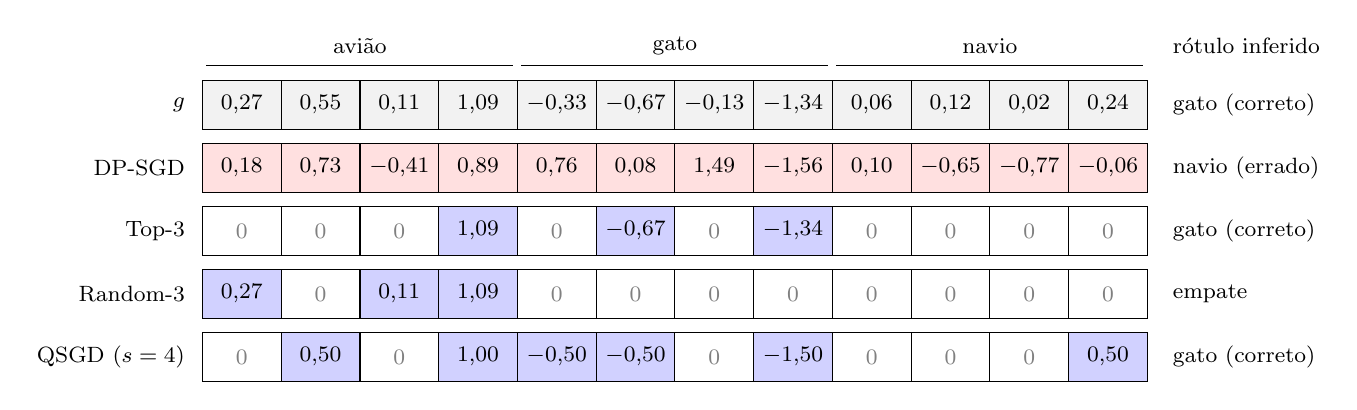
\begin{tikzpicture}[
  font=\footnotesize,
  cel/.style={draw, minimum width=1.0cm, minimum height=0.62cm, inner sep=0pt, anchor=center},
  zero/.style={cel, text=gray},
  mant/.style={cel, fill=blue!18},
  ruido/.style={cel, fill=red!12},
  lab/.style={anchor=east, font=\footnotesize},
  res/.style={anchor=west, font=\footnotesize}
]
\def\dx{1.0}\def\dy{0.8}
% cabeçalho de grupos
\foreach \nome/\ini in {avião/0, gato/4, navio/8} {
  \node[font=\footnotesize] at ({(\ini+1.5)*\dx}, 0.75) {\nome};
  \draw ({(\ini-0.45)*\dx}, 0.5) -- ({(\ini+3.45)*\dx}, 0.5);
}
\node[res] at ({11.7*\dx}, 0.75) {rótulo inferido};
% linha 1: gradiente original
\node[lab] at ({-0.6*\dx}, 0) {$g$};
\foreach \v [count=\i from 0] in {0{,}27, 0{,}55, 0{,}11, 1{,}09, $-$0{,}33, $-$0{,}67, $-$0{,}13, $-$1{,}34, 0{,}06, 0{,}12, 0{,}02, 0{,}24}
  \node[cel, fill=gray!10] at ({\i*\dx}, 0) {\v};
\node[res] at ({11.7*\dx}, 0) {gato (correto)};
% linha 2: DP-SGD
\node[lab] at ({-0.6*\dx}, -\dy) {DP-SGD};
\foreach \v [count=\i from 0] in {0{,}18, 0{,}73, $-$0{,}41, 0{,}89, 0{,}76, 0{,}08, 1{,}49, $-$1{,}56, 0{,}10, $-$0{,}65, $-$0{,}77, $-$0{,}06}
  \node[ruido] at ({\i*\dx}, -\dy) {\v};
\node[res] at ({11.7*\dx}, -\dy) {navio (errado)};
% linha 3: Top-3
\node[lab] at ({-0.6*\dx}, {-2*\dy}) {Top-3};
\foreach \v/\s [count=\i from 0] in {0/zero, 0/zero, 0/zero, 1{,}09/mant, 0/zero, $-$0{,}67/mant, 0/zero, $-$1{,}34/mant, 0/zero, 0/zero, 0/zero, 0/zero}
  \node[\s] at ({\i*\dx}, {-2*\dy}) {\v};
\node[res] at ({11.7*\dx}, {-2*\dy}) {gato (correto)};
% linha 4: Random-3
\node[lab] at ({-0.6*\dx}, {-3*\dy}) {Random-3};
\foreach \v/\s [count=\i from 0] in {0{,}27/mant, 0/zero, 0{,}11/mant, 1{,}09/mant, 0/zero, 0/zero, 0/zero, 0/zero, 0/zero, 0/zero, 0/zero, 0/zero}
  \node[\s] at ({\i*\dx}, {-3*\dy}) {\v};
\node[res] at ({11.7*\dx}, {-3*\dy}) {empate};
% linha 5: QSGD
\node[lab] at ({-0.6*\dx}, {-4*\dy}) {QSGD ($s=4$)};
\foreach \v/\s [count=\i from 0] in {0/zero, 0{,}50/mant, 0/zero, 1{,}00/mant, $-$0{,}50/mant, $-$0{,}50/mant, 0/zero, $-$1{,}50/mant, 0/zero, 0/zero, 0/zero, 0{,}50/mant}
  \node[\s] at ({\i*\dx}, {-4*\dy}) {\v};
\node[res] at ({11.7*\dx}, {-4*\dy}) {gato (correto)};
\end{tikzpicture}
\caption{Efeito das defesas sobre o gradiente do exemplo guia e rótulo inferido pela regra do iDLG. A primeira linha é o gradiente original; células em vermelho contêm ruído, células em azul são valores mantidos e zeros em cinza são valores descartados.}
\label{fig:defesas-exemplo}
\end{figure}

O exemplo resume o comportamento esperado de cada família: o ruído do DP-SGD altera todos os valores e pode inverter o padrão de sinais; o Top-$k$ preserva justamente a região mais informativa; o Random-$k$ pode ou não preservá-la, dependendo do sorteio; e o QSGD perde precisão, mas mantém os sinais. É importante lembrar que se trata de uma ilustração com um único sorteio e um modelo mínimo; o comportamento em redes reais precisa ser medido experimentalmente, com muitas repetições, o que é feito neste trabalho.

\subsubsection{Outras Técnicas de Compressão}

Outras técnicas relevantes, embora não avaliadas experimentalmente neste trabalho, completam o panorama. O SignSGD transmite apenas o sinal de cada elemento, $\mathcal{C}(g) = \mathrm{sgn}(g)$, usando um único bit por valor; é extremamente econômico, mas descarta toda a informação de magnitude \cite{Bernstein2018}. O TernGrad reduz cada elemento a três níveis, $\mathcal{C}(g) = \|g\|_\infty \cdot \mathrm{sgn}(g) \circ b$, em que $b_i$ vale $1$ com probabilidade $|g_i|/\|g\|_\infty$ e $0$ caso contrário \cite{Wen2017}. O Deep Gradient Compression (DGC) combina o Top-$k$ com o acúmulo local dos valores descartados e outras correções que preservam a acurácia mesmo com compressões muito altas \cite{Lin2018}. Por fim, a técnica de error feedback guarda o erro cometido pela compressão, $e_{t+1} = e_t + g_t - \mathcal{C}(e_t + g_t)$, e o reincorpora na rodada seguinte, corrigindo distorções de compressores como o SignSGD \cite{Karimireddy2019}.

\subsection{Métricas de Avaliação} \label{sec:metricas}

Avaliar uma defesa exige responder a duas perguntas que puxam em direções opostas. A primeira é quão difícil ficou para o adversário, o que corresponde à privacidade; a segunda é quão bom continua o modelo, o que corresponde à utilidade. As métricas a seguir quantificam cada uma delas.

\subsubsection{Erro Quadrático Médio de Reconstrução}

O erro quadrático médio (MSE) compara, pixel a pixel, a imagem original $x$ com a imagem reconstruída pelo ataque $x'$:

\begin{equation} \label{eq:mse}
\mathrm{MSE}(x, x') = \frac{1}{n} \sum_{j=1}^{n} \big( x_j - x'_j \big)^{2}
\end{equation}

\noindent onde:
\begin{description}
  \item[$x_j$, $x'_j$] = valores do pixel $j$ na imagem original e na reconstruída, na escala de intensidade dos pixels;
  \item[$n$] = número de pixels (multiplicado pelo número de canais de cor).
\end{description}

Por exemplo, para uma imagem de quatro pixels $x = (0{,}9;\ 0{,}1;\ 0{,}8;\ 0{,}2)$, uma boa reconstrução $x' = (0{,}8;\ 0{,}2;\ 0{,}8;\ 0{,}3)$ tem $\mathrm{MSE} = (0{,}01 + 0{,}01 + 0 + 0{,}01)/4 = 0{,}0075$, enquanto uma reconstrução ruim $x'' = (0{,}3;\ 0{,}7;\ 0{,}1;\ 0{,}9)$ tem $\mathrm{MSE} = (0{,}36 + 0{,}36 + 0{,}49 + 0{,}49)/4 = 0{,}425$. Portanto, MSE baixo significa vazamento, e MSE alto significa proteção. A vantagem do MSE é a simplicidade e a objetividade; sua limitação é não refletir perfeitamente a percepção humana, já que uma imagem levemente deslocada pode ter MSE alto e ainda ser reconhecível.

\subsubsection{Acurácia de Inferência de Rótulo}

A acurácia de inferência de rótulo mede em quantas das amostras atacadas o rótulo deduzido pela Equação~\ref{eq:idlg-label} estava correto:

\begin{equation} \label{eq:label-acc}
\mathrm{Acc}_{\text{rótulo}} = \frac{1}{A} \sum_{a=1}^{A} \mathbb{I}\big[\hat{c}_a = c_a\big]
\end{equation}

\noindent onde:
\begin{description}
  \item[$A$] = número de amostras atacadas;
  \item[$\hat{c}_a$, $c_a$] = rótulo inferido e rótulo verdadeiro da amostra $a$.
\end{description}

Se o ataque acerta o rótulo de 9 entre 10 amostras, a métrica vale $90\%$. Em um problema com dez classes, um adversário que chuta ao acaso acerta cerca de $10\%$; valores próximos desse patamar indicam que a defesa escondeu o rótulo. Essa métrica é relevante porque, mesmo quando a imagem não é reconstruída, o rótulo já pode ser uma informação sensível, como um diagnóstico.

\subsubsection{Acurácia de Teste}

A utilidade é medida pela acurácia no conjunto de teste, isto é, a proporção de imagens não vistas no treinamento que o modelo classifica corretamente:

\begin{equation} \label{eq:acc}
\mathrm{Acc}_{\text{teste}} = \frac{1}{N_{\text{teste}}} \sum_{i=1}^{N_{\text{teste}}} \mathbb{I}\Big[\arg\max_j f_\theta(x_i)_j = y_i\Big]
\end{equation}

\noindent onde $\arg\max_j f_\theta(x_i)_j$ é a classe com maior probabilidade prevista pelo modelo. Se um modelo acerta 426 de 1.000 imagens de teste, sua acurácia é $0{,}426$. Uma boa defesa deve aumentar o MSE e reduzir a acurácia de inferência de rótulo sem derrubar a acurácia de teste.

\subsubsection{Teste $t$ de Welch e Tamanho de Efeito}

Como os resultados variam a cada execução, por causa dos sorteios de inicialização, lotes e ruído, não basta comparar duas médias: é preciso verificar se a diferença é maior do que a variação natural. O teste $t$ de Welch compara as médias de dois grupos independentes sem supor que tenham a mesma variabilidade \cite{Welch1947}:

\begin{equation} \label{eq:welch}
t = \frac{\bar{x}_1 - \bar{x}_2}{\sqrt{\dfrac{s_1^2}{n_1} + \dfrac{s_2^2}{n_2}}}, \qquad
\nu \approx \frac{\left( \dfrac{s_1^2}{n_1} + \dfrac{s_2^2}{n_2} \right)^{2}}{\dfrac{(s_1^2/n_1)^2}{n_1 - 1} + \dfrac{(s_2^2/n_2)^2}{n_2 - 1}}
\end{equation}

\noindent onde:
\begin{description}
  \item[$\bar{x}_g$, $s_g^2$, $n_g$] = média, variância e tamanho do grupo $g$;
  \item[$\nu$] = graus de liberdade aproximados, usados para obter o valor-$p$.
\end{description}

O valor-$p$ indica a probabilidade de observar uma diferença tão grande quanto a encontrada se, na verdade, não houvesse diferença alguma. Quando ele é menor que o nível de significância $\alpha$, tipicamente $0{,}05$, conclui-se que a diferença é estatisticamente significativa. Contudo, uma diferença pode ser significativa e, ainda assim, pequena. Para medir seu tamanho, utiliza-se o $d$ de Cohen \cite{Cohen1988}:

\begin{equation} \label{eq:cohen}
d = \frac{\bar{x}_1 - \bar{x}_2}{s_p}, \qquad s_p = \sqrt{\frac{(n_1 - 1)s_1^2 + (n_2 - 1)s_2^2}{n_1 + n_2 - 2}}
\end{equation}

\noindent em que $s_p$ é o desvio-padrão combinado dos dois grupos. Valores de $|d|$ próximos de $0{,}2$, $0{,}5$ e $0{,}8$ são interpretados, respectivamente, como efeitos pequeno, médio e grande.

Como exemplo, suponha cinco medições de MSE sem defesa, $(0{,}009;\ 0{,}004;\ 0{,}012;\ 0{,}007;\ 0{,}015)$, com média $0{,}0094$ e desvio-padrão $0{,}0043$, e cinco medições com uma defesa, $(0{,}090;\ 0{,}020;\ 0{,}150;\ 0{,}060;\ 0{,}110)$, com média $0{,}086$ e desvio-padrão $0{,}049$. O teste de Welch resulta em $t = -3{,}46$, com $\nu \approx 4{,}1$ graus de liberdade e valor-$p \approx 0{,}025$, menor que $0{,}05$: a defesa aumentou o MSE de forma significativa. O $d$ de Cohen vale $-2{,}19$, indicando um efeito grande. Com apenas cinco medições por grupo, porém, o teste tem pouca sensibilidade; por isso, este trabalho utiliza até 30 observações por configuração, correspondentes a 30 execuções de treinamento na avaliação da acurácia e a 30 imagens atacadas na avaliação do MSE.

% =====================================================================
\section{Trabalhos Relacionados} \label{sec:relacionados}
% =====================================================================

Esta seção descreve os principais trabalhos que fundamentam e motivam a presente pesquisa, organizados em três eixos: o vazamento de privacidade em aprendizado colaborativo, os ataques de reconstrução a partir de gradientes e as defesas e suas avaliações empíricas. Para cada trabalho, apresentam-se o contexto, os métodos empregados e os resultados alcançados. Ao final, a proposta deste trabalho é comparada aos estudos descritos.

\subsection{Vazamento de Privacidade em Aprendizado Colaborativo}

\citeonline{Shokri2015} propuseram um dos primeiros sistemas de aprendizado profundo colaborativo com preservação de privacidade, o Distributed Selective SGD. Nesse sistema, participantes treinam modelos locais e compartilham apenas uma fração selecionada dos gradientes, escolhida pelas maiores magnitudes ou aleatoriamente, podendo ainda adicionar ruído diferencialmente privado. Experimentos em MNIST e SVHN mostraram que o compartilhamento de uma pequena fração dos parâmetros permitia atingir acurácia próxima à do treinamento centralizado. O trabalho é relevante por antecipar, com propósito de privacidade, as mesmas operações de seleção Top-$k$ e aleatória avaliadas nesta pesquisa.

\citeonline{McMahan2017} formalizaram o aprendizado federado e propuseram o FedAvg (Algoritmo~\ref{alg:fedavg}). Em experimentos com MNIST e com modelos de linguagem sobre textos de Shakespeare, sob partições de dados não independentes e identicamente distribuídas, o FedAvg reduziu o número de rodadas de comunicação em uma a duas ordens de grandeza em relação ao FedSGD. Os autores apontaram a privacidade como motivação central, argumentando que as atualizações contêm menos informação que os dados brutos, mas sem quantificar o vazamento remanescente.

\citeonline{Melis2019} demonstraram que essa informação remanescente é explorável. Analisando as atualizações trocadas em aprendizado colaborativo, construíram ataques de inferência de pertinência (membership inference) e de propriedades, capazes de detectar se determinado exemplo foi usado no treinamento e de inferir atributos não relacionados à tarefa principal, como características de pessoas em fotografias. Os resultados evidenciaram que os gradientes revelam mais do que o necessário para a tarefa, fenômeno denominado vazamento não intencional de atributos.

\citeonline{Kairouz2021} consolidaram, em ampla revisão, os avanços e problemas em aberto do aprendizado federado. O trabalho sistematiza modelos de ameaça, técnicas criptográficas como a agregação segura \cite{Bonawitz2017}, privacidade diferencial nos níveis local e central e compressão de comunicação, destacando a necessidade de avaliar conjuntamente privacidade, eficiência e utilidade.

\subsection{Ataques de Reconstrução a partir de Gradientes}

\citeonline{Zhu2019} apresentaram o DLG, primeiro ataque a reconstruir imagens e textos com fidelidade de pixel e de token a partir de gradientes. O método otimiza entradas e rótulos sintéticos para coincidir com o gradiente observado (Equação~\ref{eq:dlg}), usando L-BFGS. Em experimentos com uma LeNet modificada sobre MNIST, CIFAR-100, SVHN e LFW, o ataque recuperou imagens praticamente idênticas às originais em poucas centenas de iterações, inclusive para lotes de até oito imagens. Os autores avaliaram também defesas simples: ruído gaussiano ou laplaciano com variância a partir de $10^{-2}$ impediu a reconstrução, mas com degradação acentuada da acurácia; a representação em meia precisão não ofereceu proteção; e a poda de gradientes de pequena magnitude tornou as reconstruções irreconhecíveis a partir de cerca de 20\% de esparsidade. Essas observações preliminares, obtidas em uma única arquitetura, motivam a avaliação sistemática realizada neste trabalho.

\citeonline{Zhao2020} propuseram o iDLG ao identificarem que o DLG frequentemente converge para rótulos incorretos. A partir da análise do sinal do gradiente da última camada sob entropia cruzada (Equações~\ref{eq:grad-logit} e \ref{eq:idlg-label}), demonstraram que o rótulo de uma única amostra pode ser extraído analiticamente com 100\% de acerto. Em MNIST, CIFAR-100 e LFW, a extração prévia do rótulo aumentou a taxa de sucesso da reconstrução e acelerou a convergência em relação ao DLG.

\citeonline{Geiping2020} investigaram o quão realista é a ameaça em cenários próximos aos de implantação. Propuseram a função de custo baseada em similaridade de cossenos com regularização TV (Equação~\ref{eq:ig}) e demonstraram analiticamente que a entrada de uma camada totalmente conectada pode ser recuperada exatamente de seu gradiente. Os experimentos, com redes ResNet treinadas e não treinadas sobre CIFAR-10 e ImageNet, mostraram reconstruções reconhecíveis de imagens de alta resolução, recuperação parcial de imagens em lotes maiores e vazamento mesmo quando os clientes executam múltiplos passos locais, como no FedAvg. Os autores concluíram que a agregação de gradientes, por si só, não garante privacidade.

\citeonline{Yin2021} ampliaram a escala dos ataques com o GradInversion, que recupera lotes de imagens do ImageNet a partir de gradientes de uma ResNet-50. O método combina a restauração de rótulos do lote a partir da camada totalmente conectada, uma regularização de fidelidade baseada nas estatísticas das camadas de normalização em lote e um termo de consistência entre múltiplas reconstruções. Foram obtidas reconstruções detalhadas para lotes de até 48 imagens, evidenciando que lotes grandes não constituem, isoladamente, uma defesa suficiente.

\subsection{Defesas e Avaliações Empíricas}

\citeonline{Abadi2016} propuseram o DP-SGD (Algoritmo~\ref{alg:dpsgd}) e o moments accountant, viabilizando o treinamento de redes profundas com garantias formais de privacidade diferencial sob orçamentos moderados. Com $\delta = 10^{-5}$, os autores relataram acurácias de aproximadamente 90\%, 95\% e 97\% no MNIST para $\varepsilon$ igual a $0{,}5$, $2$ e $8$, e de 73\% no CIFAR-10 para $\varepsilon = 8$, abaixo dos valores obtidos sem privacidade. O trabalho quantificou o custo de utilidade da privacidade diferencial, mas não avaliou a resistência empírica a ataques de inversão, que foram propostos posteriormente.

\citeonline{McMahan2018} estenderam a privacidade diferencial ao aprendizado federado no nível do usuário com o DP-FedAvg, aplicando-o a modelos recorrentes de linguagem. Mostraram que, com um número suficientemente grande de usuários por rodada, é possível obter garantias formais com perda de acurácia pequena, à custa de maior computação. O resultado indica que o custo da privacidade diferencial depende fortemente da escala da federação, aspecto ausente em cenários com poucos clientes.

\citeonline{Wei2020} propuseram um arcabouço para avaliar o vazamento de dados de clientes em aprendizado federado frente a ataques de reconstrução por gradientes. Analisaram sistematicamente o efeito da inicialização do ataque, do tamanho do lote, da frequência de comunicação e do estágio do treinamento, e avaliaram defesas baseadas em adição de ruído e em compressão de gradientes em múltiplas bases de dados. Os resultados indicaram que a eficácia do ataque é sensível a esses fatores e que as defesas oferecem proteção variável conforme sua configuração, reforçando a necessidade de protocolos padronizados de avaliação.

\citeonline{Sun2021} propuseram o Soteria, defesa que perturba a representação dos dados em uma camada totalmente conectada escolhida, em vez de perturbar o gradiente de toda a rede. A perturbação é calculada para maximizar a distância entre a entrada original e a reconstruída, com restrição sobre o impacto na representação, e é acompanhada de análise teórica de convergência para o FedAvg. Em experimentos com MNIST e CIFAR-10 contra DLG e Inverting Gradients, o Soteria degradou a qualidade das reconstruções mantendo acurácia próxima à do modelo sem defesa.

\citeonline{Huang2021} avaliaram criticamente ataques e defesas de inversão de gradientes em CIFAR-10 com ResNet-18. Mostraram que parte do sucesso reportado pelos ataques decorre de hipóteses fortes, como o conhecimento das estatísticas de normalização em lote e dos rótulos, e avaliaram defesas como poda de gradientes, MixUp e InstaHide, isoladamente e combinadas. Concluíram que a poda com taxas elevadas, especialmente combinada a outras técnicas, pode reduzir substancialmente o vazamento com perda moderada de acurácia, e recomendaram que as defesas sejam avaliadas sempre em conjunto com seu custo de utilidade.

As técnicas de compressão Top-$k$ com memória \cite{Stich2018}, Random-$k$ \cite{Wangni2018}, QSGD \cite{Alistarh2017}, SignSGD \cite{Bernstein2018}, TernGrad \cite{Wen2017}, DGC \cite{Lin2018} e error feedback \cite{Karimireddy2019} foram propostas e avaliadas com foco em eficiência de comunicação. \citeonline{Lin2018}, por exemplo, observaram que a maior parte da troca de gradientes em treinamento distribuído é redundante e obtiveram taxas de compressão de 270 a 600 vezes sem perda de acurácia em classificação de imagens, reconhecimento de fala e modelagem de linguagem. Esses trabalhos, contudo, não investigam o efeito da compressão sobre ataques de inversão, deixando em aberto se a redução de informação voltada à eficiência também se traduz em proteção.

\subsection{Síntese e Posicionamento deste Trabalho} \label{sec:posicionamento}

A análise da literatura permite identificar três lacunas. Primeiro, a maior parte dos trabalhos de ataque \cite{Zhu2019,Zhao2020,Geiping2020,Yin2021} demonstra a vulnerabilidade, mas avalia defesas de forma incidental, com uma única arquitetura e sem medir sistematicamente o custo de utilidade. Segundo, os trabalhos de defesa baseados em privacidade diferencial \cite{Abadi2016,McMahan2018} quantificam a utilidade sob garantias formais, mas não a resistência empírica a ataques de inversão; já as técnicas de compressão \cite{Stich2018,Wangni2018,Alistarh2017,Lin2018} foram concebidas para eficiência de comunicação, sem avaliação de privacidade. Terceiro, as avaliações comparativas existentes \cite{Wei2020,Huang2021} concentram-se em arquiteturas convolucionais e em conjuntos específicos de defesas, não confrontando, sob um mesmo protocolo, privacidade diferencial e as diferentes famílias de compressão, nem arquiteturas baseadas em atenção como o ViT.

Assim como \citeonline{Zhu2019} e \citeonline{Huang2021}, este trabalho avalia defesas contra ataques de inversão e considera o custo de utilidade; assim como \citeonline{Zhao2020}, adota o iDLG, que representa um adversário capaz de inferir o rótulo analiticamente. O primeiro diferencial da proposta é comparar, sob um protocolo fatorial único, cinco configurações que abrangem as duas principais famílias de defesa: ausência de defesa, DP-SGD, Top-$k$, Random-$k$ e QSGD. Além disso, o estudo inclui três arquiteturas com vieses indutivos distintos, MLP, CNN e ViT, e três bases de dados de complexidade crescente. A privacidade é medida de forma conjunta com a utilidade, a primeira pelo MSE de reconstrução e pela acurácia de inferência de rótulo e a segunda pela acurácia de teste. Por fim, a utilidade de cada configuração é medida em 30 execuções com sementes distintas, a privacidade é medida sobre 30 imagens atacadas, e as comparações são sustentadas por testes estatísticos e tamanhos de efeito. Em contrapartida, o estudo adota um cenário de cliente único, sem agregação FedAvg, que corresponde ao caso mais favorável ao adversário discutido na Seção~\ref{sec:fl}, e aplica o DP-SGD como mecanismo empírico de ruído, sem contabilização formal do orçamento $(\varepsilon, \delta)$. Técnicas como privacidade diferencial no nível do cliente, LDP, SignSGD, TernGrad, DGC e error feedback foram apresentadas na fundamentação teórica, mas permanecem fora do escopo experimental.
